\chapter{Análisis y diseño}\label{chp:introduccion}

En este capítulo se describe el análisis y el diseño del trabajo propuesto para
la recolección, clasificación de noticias y el entorno web.

\section{Requisitos funcionales}

%----------------------------RF1------------------------------%
   \Dline{RF1}{Recolectar noticias}
    \begin{itemize}
      \item \textbf{Descripción:} El sistema debe recolectar noticias de forma automática en la internet\\
    \end{itemize}
%----------------------------RF2------------------------------%
   \Dline{RF2}{Clasificar noticias}
    \begin{itemize}
      \item \textbf{Descripción:} El sistema debe clasificar las noticias recolectadas deacuerdo a su contenido\\
    \end{itemize}
%----------------------------RF3------------------------------%
   \Dline{RF3}{Filtrar por fehca}
    \begin{itemize}
      \item \textbf{Descripción:} El sistema debe permitir filtrar las noticias deacuerdo a su fecha de publicación\\
    \end{itemize}
%----------------------------RF4------------------------------%
   \Dline{RF4}{Entorno web}
    \begin{itemize}
      \item \textbf{Descripción:} El sistema debe mostrar las noticias recolectadas y clasificadas al usuario en un entorno web\\
    \end{itemize}
%----------------------------RF5------------------------------%
   \Dline{RF5}{Link a noticia}
    \begin{itemize}
      \item \textbf{Descripción:} Cada noticia mostrada debe contener un hipervínculo que rediriga al usuario a su sitio de origen\\
    \end{itemize}


%----------------------------Requisito no funcionales---------------------------%  

\section{Requisitos No funcionales}

%----------------------------RNF1------------------------------%
   \DVline{RNF1}{Tiempo de clasificación}
    \begin{itemize}
      \item \textbf{Descripción:} La clasificación de una noticia no debe tardar mas de un segundo\\
    \end{itemize}

%----------------------------RNF2------------------------------%
   \DVline{RNF2}{Número de palabras}
    \begin{itemize}
     \item \textbf{Descripción:} Las noticias recolectads deberán tener un mínimo de 180 palabras en ellas\\
    \end{itemize}

%----------------------------RNF3------------------------------%  
   \DVline{RNF3}{Número de noticias mostradas}
    \begin{itemize}
      \item \textbf{Descripción:} En el sitio web, se den visualizar almenos 15 noticias\\
    \end{itemize}

%----------------------------RNF4------------------------------%  
   \DVline{RNF4}{Tiempo de actualización}
    \begin{itemize}
      \item \textbf{Descripción:} El tiempo para mostrar las 15 noticias clasificadas no debe exceder los 3 segundos\\
    \end{itemize}


%----------------------------Reglas de negocio------------------------------%  

\section{Reglas de negocio}
  
  En esta sección se describen las reglas de negocio implementadas en el trabajo propuesto.\\\\


%------------------RN1-----------------------%
  \DGline{RN1}{Número de palabras}
  \begin{itemize}
    \item \textbf{Tipo:}  
    \item \textbf{Descripción:}  La notica debe tener almenos 180 palabras
    \item \textbf{Ejemplo:}
    \item \textbf{Referenciado por:} nombre caso de uso \\
  \end{itemize}

%------------------RN2-----------------------%
  \DGline{RN2}{Lenguaje}

  \begin{itemize}
    \item \textbf{Tipo:}  
    \item \textbf{Descripción:}  Las noticias deben estar redactadas en lenguaje español
    \item \textbf{Ejemplo:}
    \item \textbf{Referenciado por:} nombre caso de uso \\
  \end{itemize}


  %--------------------------Casos de uso -------------------------%

\newpage
\section{Casos de uso}


\subsection{Diagrama de casos de uso}
La figura \ref{fig:DCU} muestra el diagrama de casos de uso implementado en el sistema.

\begin{figure}[h]
  \centering
  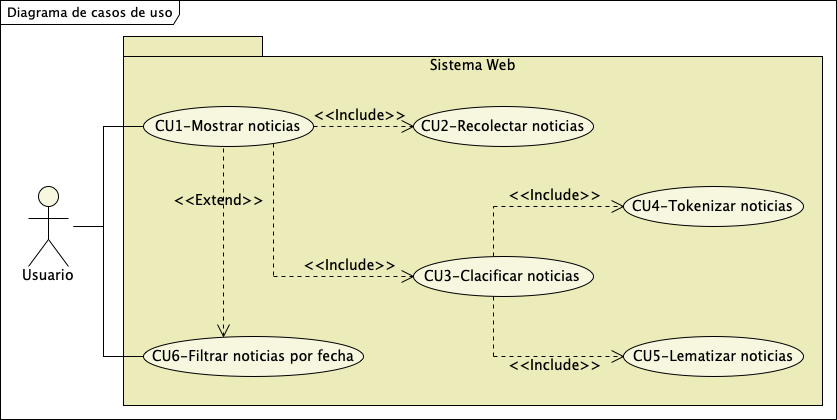
\includegraphics[scale=.4]{imagenes/Diagramas/CasosDeuso}
  \caption{Diagrama de casos de uso}
  \label{fig:DCU}
\end{figure}

{\setlength{\parindent}{0pt}%Con este comando eliminos la indexación de cada párrafo%

  \input{Capitulos/CasosDeUso/cu1-mostrarNoticia}
  \newpage
  \input{Capitulos/CasosDeUso/cu2-recolectarNoticias}
  \newpage
  \input{Capitulos/CasosDeUso/cu3-clasificarNoticia}
  \newpage
  \input{Capitulos/CasosDeUso/cu4-tokenizarNoticias}
  \newpage
  \Tsubsection{CU5 Lematizar noticias}

\begin{large}
	\textbf{Resumen}\\
\end{large}

Texto.\\

\begin{large}
	\textbf{Descripción}\\
\end{large}

\begin{tabular}{|l|l|}
	\hline
	\multicolumn{1}{| >{\columncolor{black}}l|}{ \textcolor{myWhite}{\textbf{Caso de uso: }} }&
	\multicolumn{1}{| >{\columncolor{black}}l|}{ \textcolor{myWhite}{CU-1 Recolectar noticias} }\\
	\hline
	\textbf{Actor:} & 	Lorem Ipsum	\\
	\hline
	\textbf{Propósito:} & Lorem Ipsum \\
	\hline
	\textbf{Entradas:} & Lorem Ipsum \\
	\hline
	\textbf{Salidas:} & Lorem Ipsum\\
	\hline
	\textbf{Precondición:} & Lorem Ipsum \\
	\hline
	\textbf{Postcondiciones:} & Lorem Ipsum \\
	\hline
	\textbf{Reglas de negocio:} & Lorem Ipsum \\
	\hline
	\textbf{Errores:} & Lorem Ipsum \\
	\hline
	\textbf{Autor:} & Lorem Ipsum \\
	\hline
\end{tabular}\\\\

%--------------------Trayectoria Principal-----------%


\begin{large}
	\textbf{Trayectoria principal}\\
\end{large}	

\begin{enumerate}[1.]
	\item \actor lorem ipsum
	\item \sistema lorem ipsum
	\item \sistema lorem ipsum
	\item \sistema lorem ipsum
	\item \finCU	
\end{enumerate}


%--------------------trayectoria Alternatia A---------%

\begin{large}
	\textbf{Trayectoria alternativa A:}\\
\end{large}	
\textbf{Condición:} \textit{Se escribe la condición}
\begin{enumerate}[{A-}1.]

	\item \actor lorem ipsum
	\item \sistema lorem ipsum
	\item \finTA	

\end{enumerate}


%--------------------trayectoria Alternatia b---------%
\begin{large}
	\textbf{Trayectoria alternativa B:}\\
\end{large}	
\textbf{Condición:} \textit{Se escribe la condición}

\begin{enumerate}[{B-}1.]

	\item \actor lorem ipsum
	\item \sistema lorem ipsum
	\item \finTA	

\end{enumerate}


%--------------------Puntos de extención--------------------%

\begin{large}
	\textbf{Puntos de extensión}\\
\end{large}	

\textbf{Causa de la extensión:} Lorem ipsum\\
\textbf{Región de la trayectorioa:} Lorem ipsum\\
\textbf{Extiende a :} Lorem ipsum\\\\

\textbf{Causa de la extensión:} Lorem ipsum\\
\textbf{Región de la trayectorioa:} Lorem ipsum\\
\textbf{Extiende a :} Lorem ipsum\\


  \newpage
  \input{Capitulos/CasosDeUso/cu6-FiltrarNoticiaFecha}
  \newpage
}
  %--------------------------Descripción de pantallas ------------------%
\section{Pantallas}

\input{Capitulos/CasosDeUso/DescripcionPantallas/ui1-inicio}
\newpage
\subsection{UI2-Sección deportes}

\Large{\textbf{Objetivo}}\\\\
\normalsize{Texto}\\



\Large{\textbf{Descripción}}\\
\normalsize{Texto}\\


\Large{\textbf{Comandos}}\\
\normalsize{}

\begin{itemize}
	\item Lorem ipsum
	\item Lorem ipsum
	\item Lorem ipsum
\end{itemize}

\Large{\textbf{Referencia}}\\\\
\normalsize{Nombre Caso de uso}

\begin{figure}
  \centering
	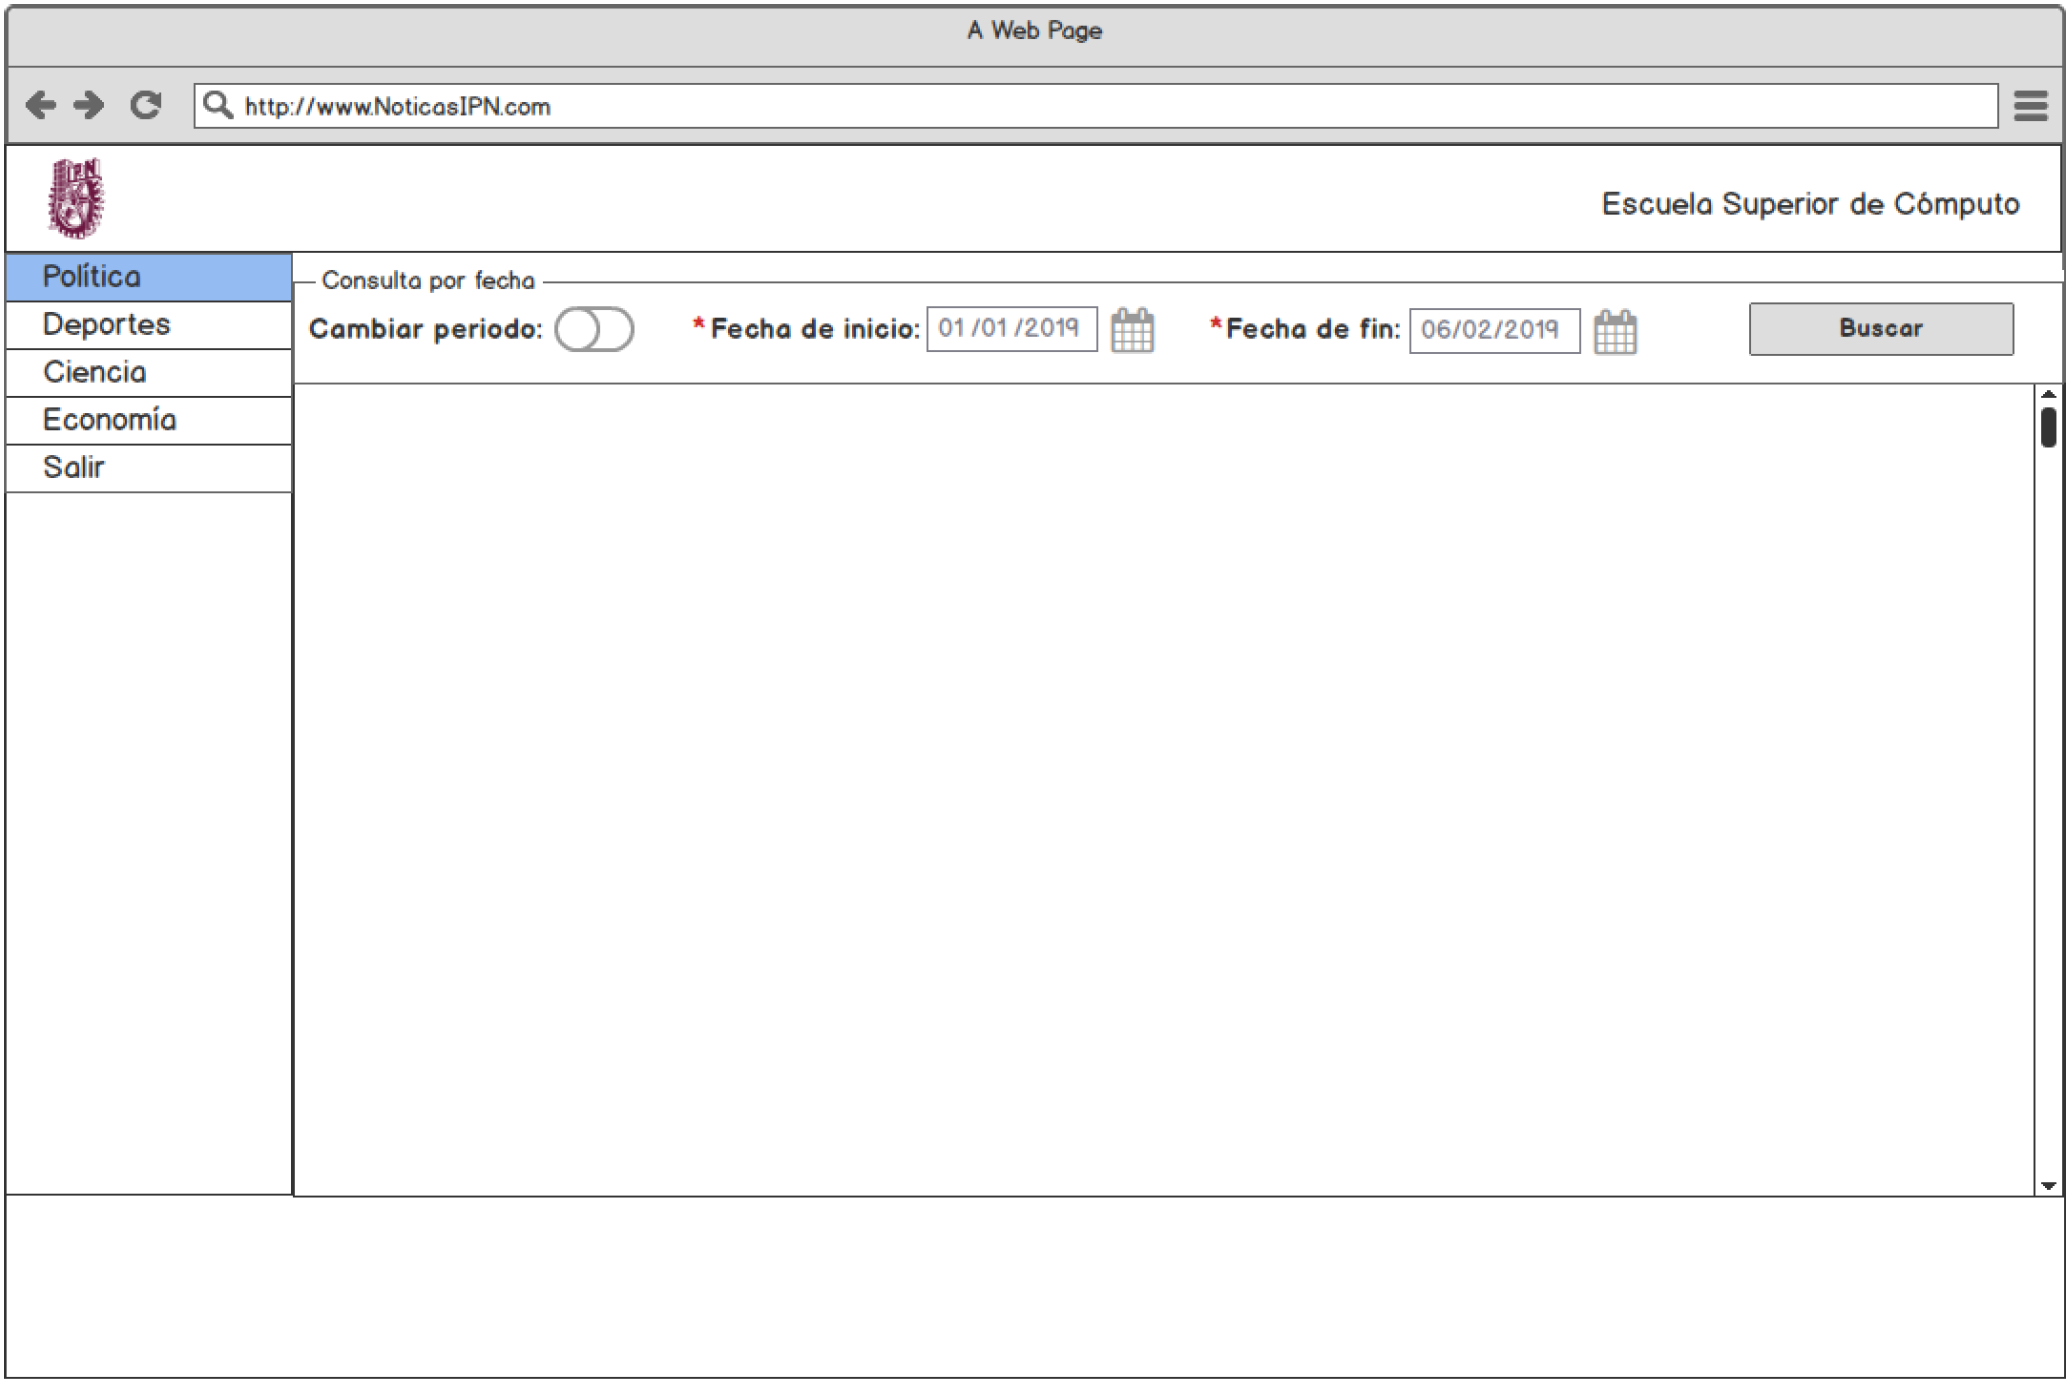
\includegraphics[scale=.3]{imagenes/Pantallas/UI2}
  \caption{Pantalla IU2-Sección deportes}
  \label{fig:IU2}
\end{figure}
\newpage
\subsection{UI3-Busqueda por fecha}

\Large{\textbf{Objetivo}}\\\\
\normalsize{Texto}\\

	

\Large{\textbf{Descripción}}\\
\normalsize{Texto}\\



\Large{\textbf{Comandos}}\\
\normalsize{}

\begin{itemize}
	\item Lorem ipsum
	\item Lorem ipsum
	\item Lorem ipsum
\end{itemize}

\Large{\textbf{Referencia}}\\\\
\normalsize{Nombre Caso de uso}

\begin{figure}[h]
  \centering
	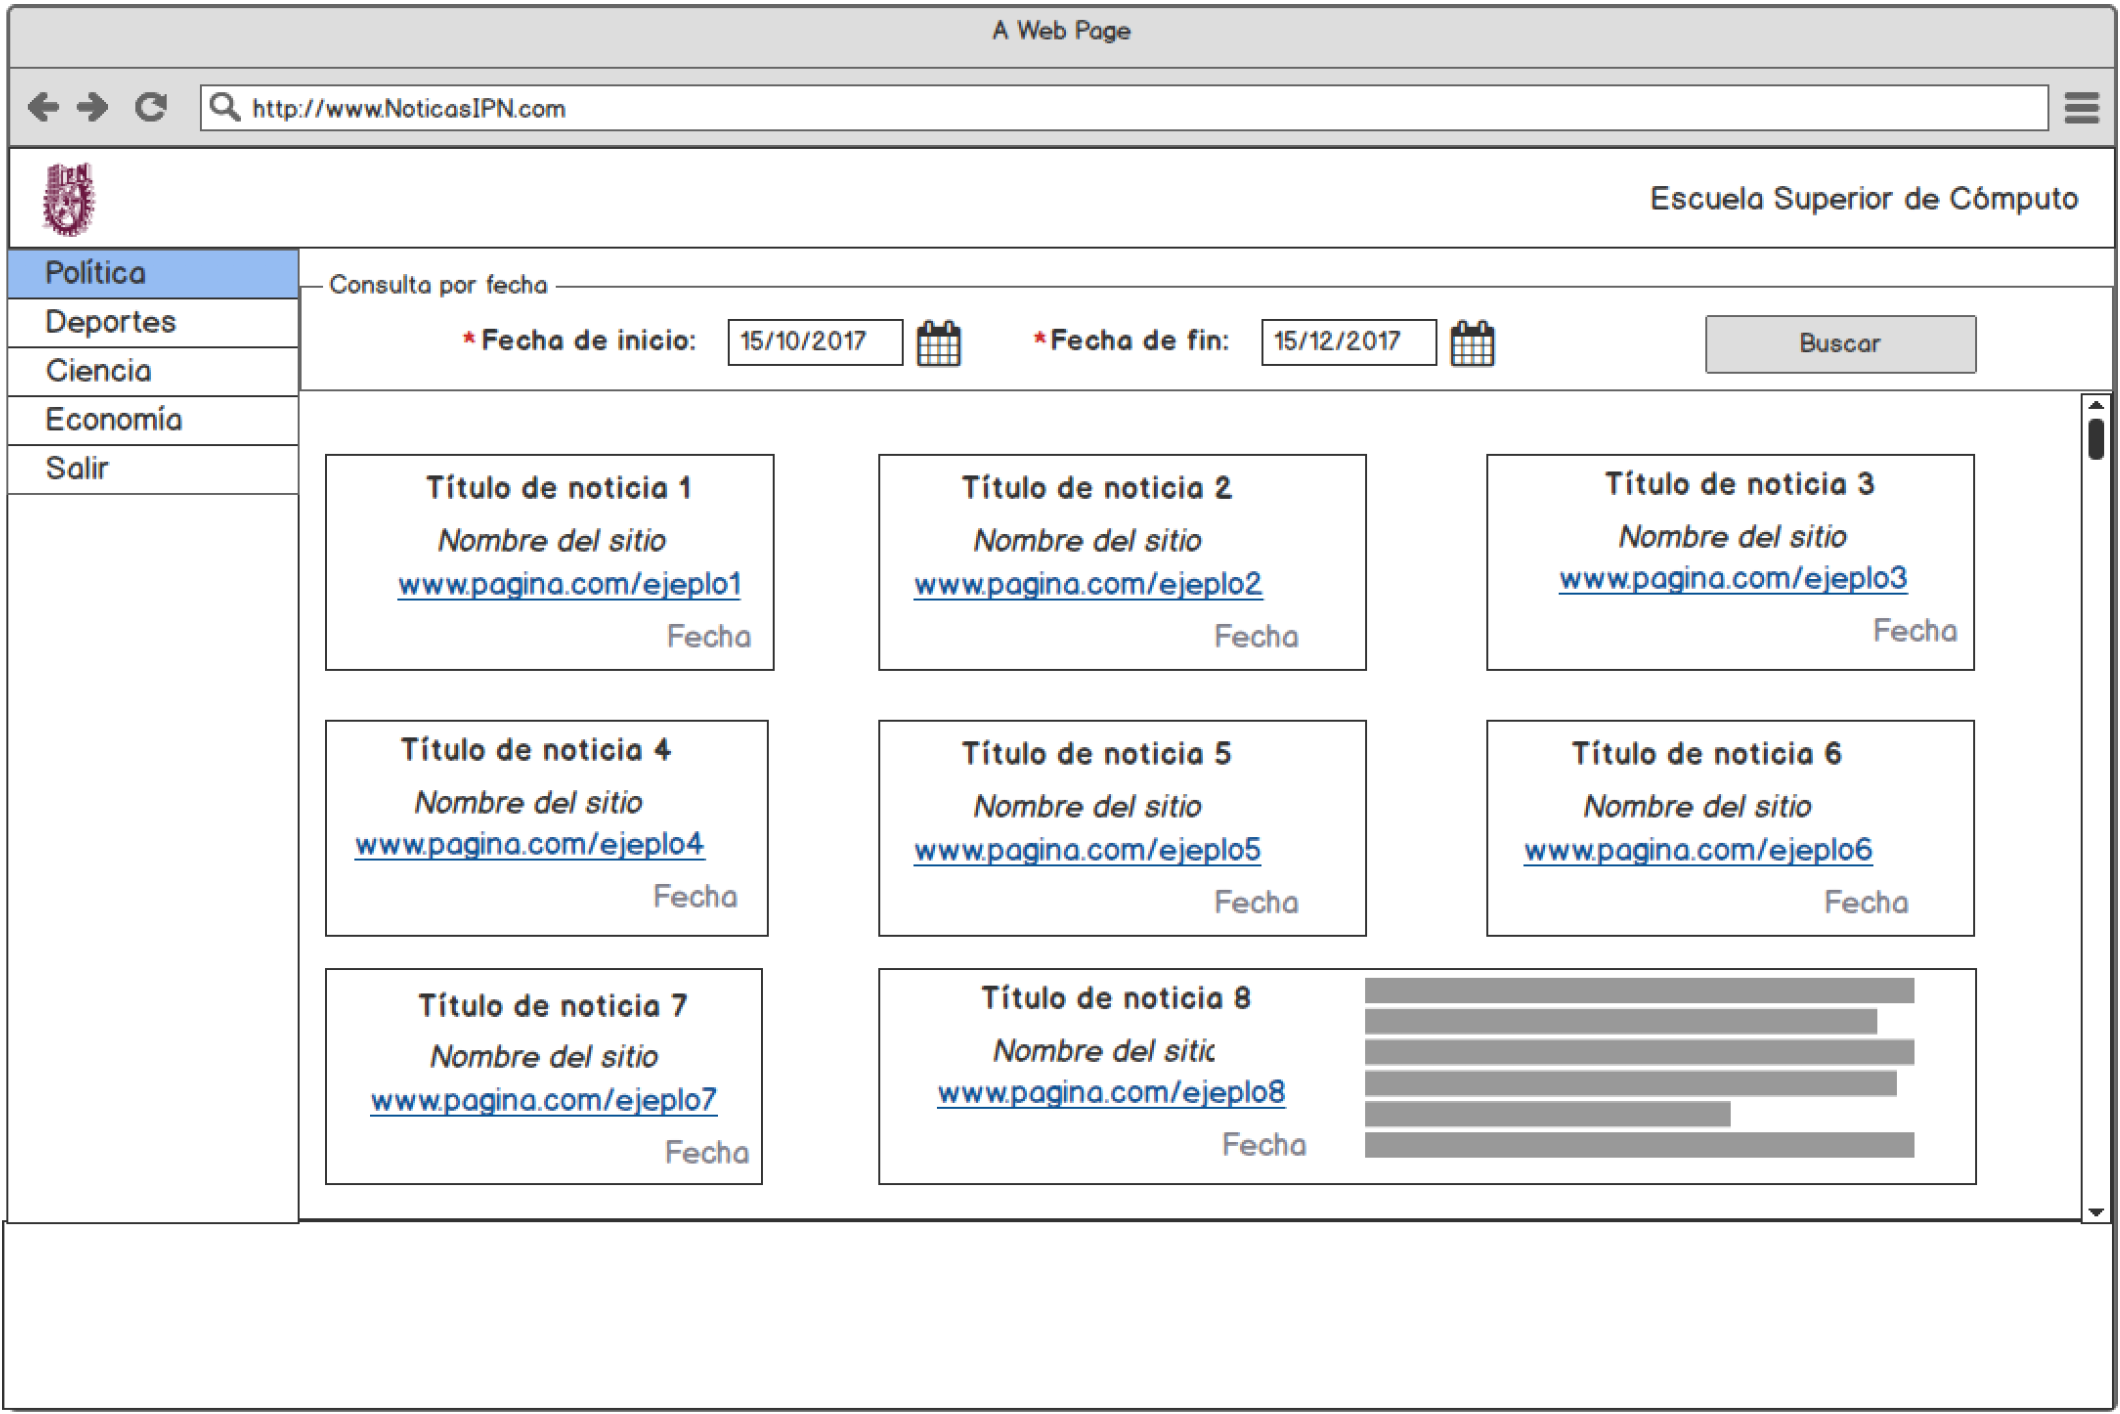
\includegraphics[scale=.3]{imagenes/Pantallas/UI3}
  \caption{Pantalla IU3-Busqueda por fecha}
  \label{fig:IU3}
\end{figure}
\newpage
\subsection{UI4-Página ejemplo}

\Large{\textbf{Objetivo}}\\\\
\normalsize{Texto}\\



\Large{\textbf{Descripción}}\\
\normalsize{Texto}\\


\Large{\textbf{Comandos}}\\
\normalsize{Texto}

\begin{itemize}
	\item Lorem ipsum
	\item Lorem ipsum
	\item Lorem ipsum
\end{itemize}

\Large{\textbf{Referencia}}\\\\
\normalsize{Nombre Caso de uso}

\begin{figure}
  \centering
	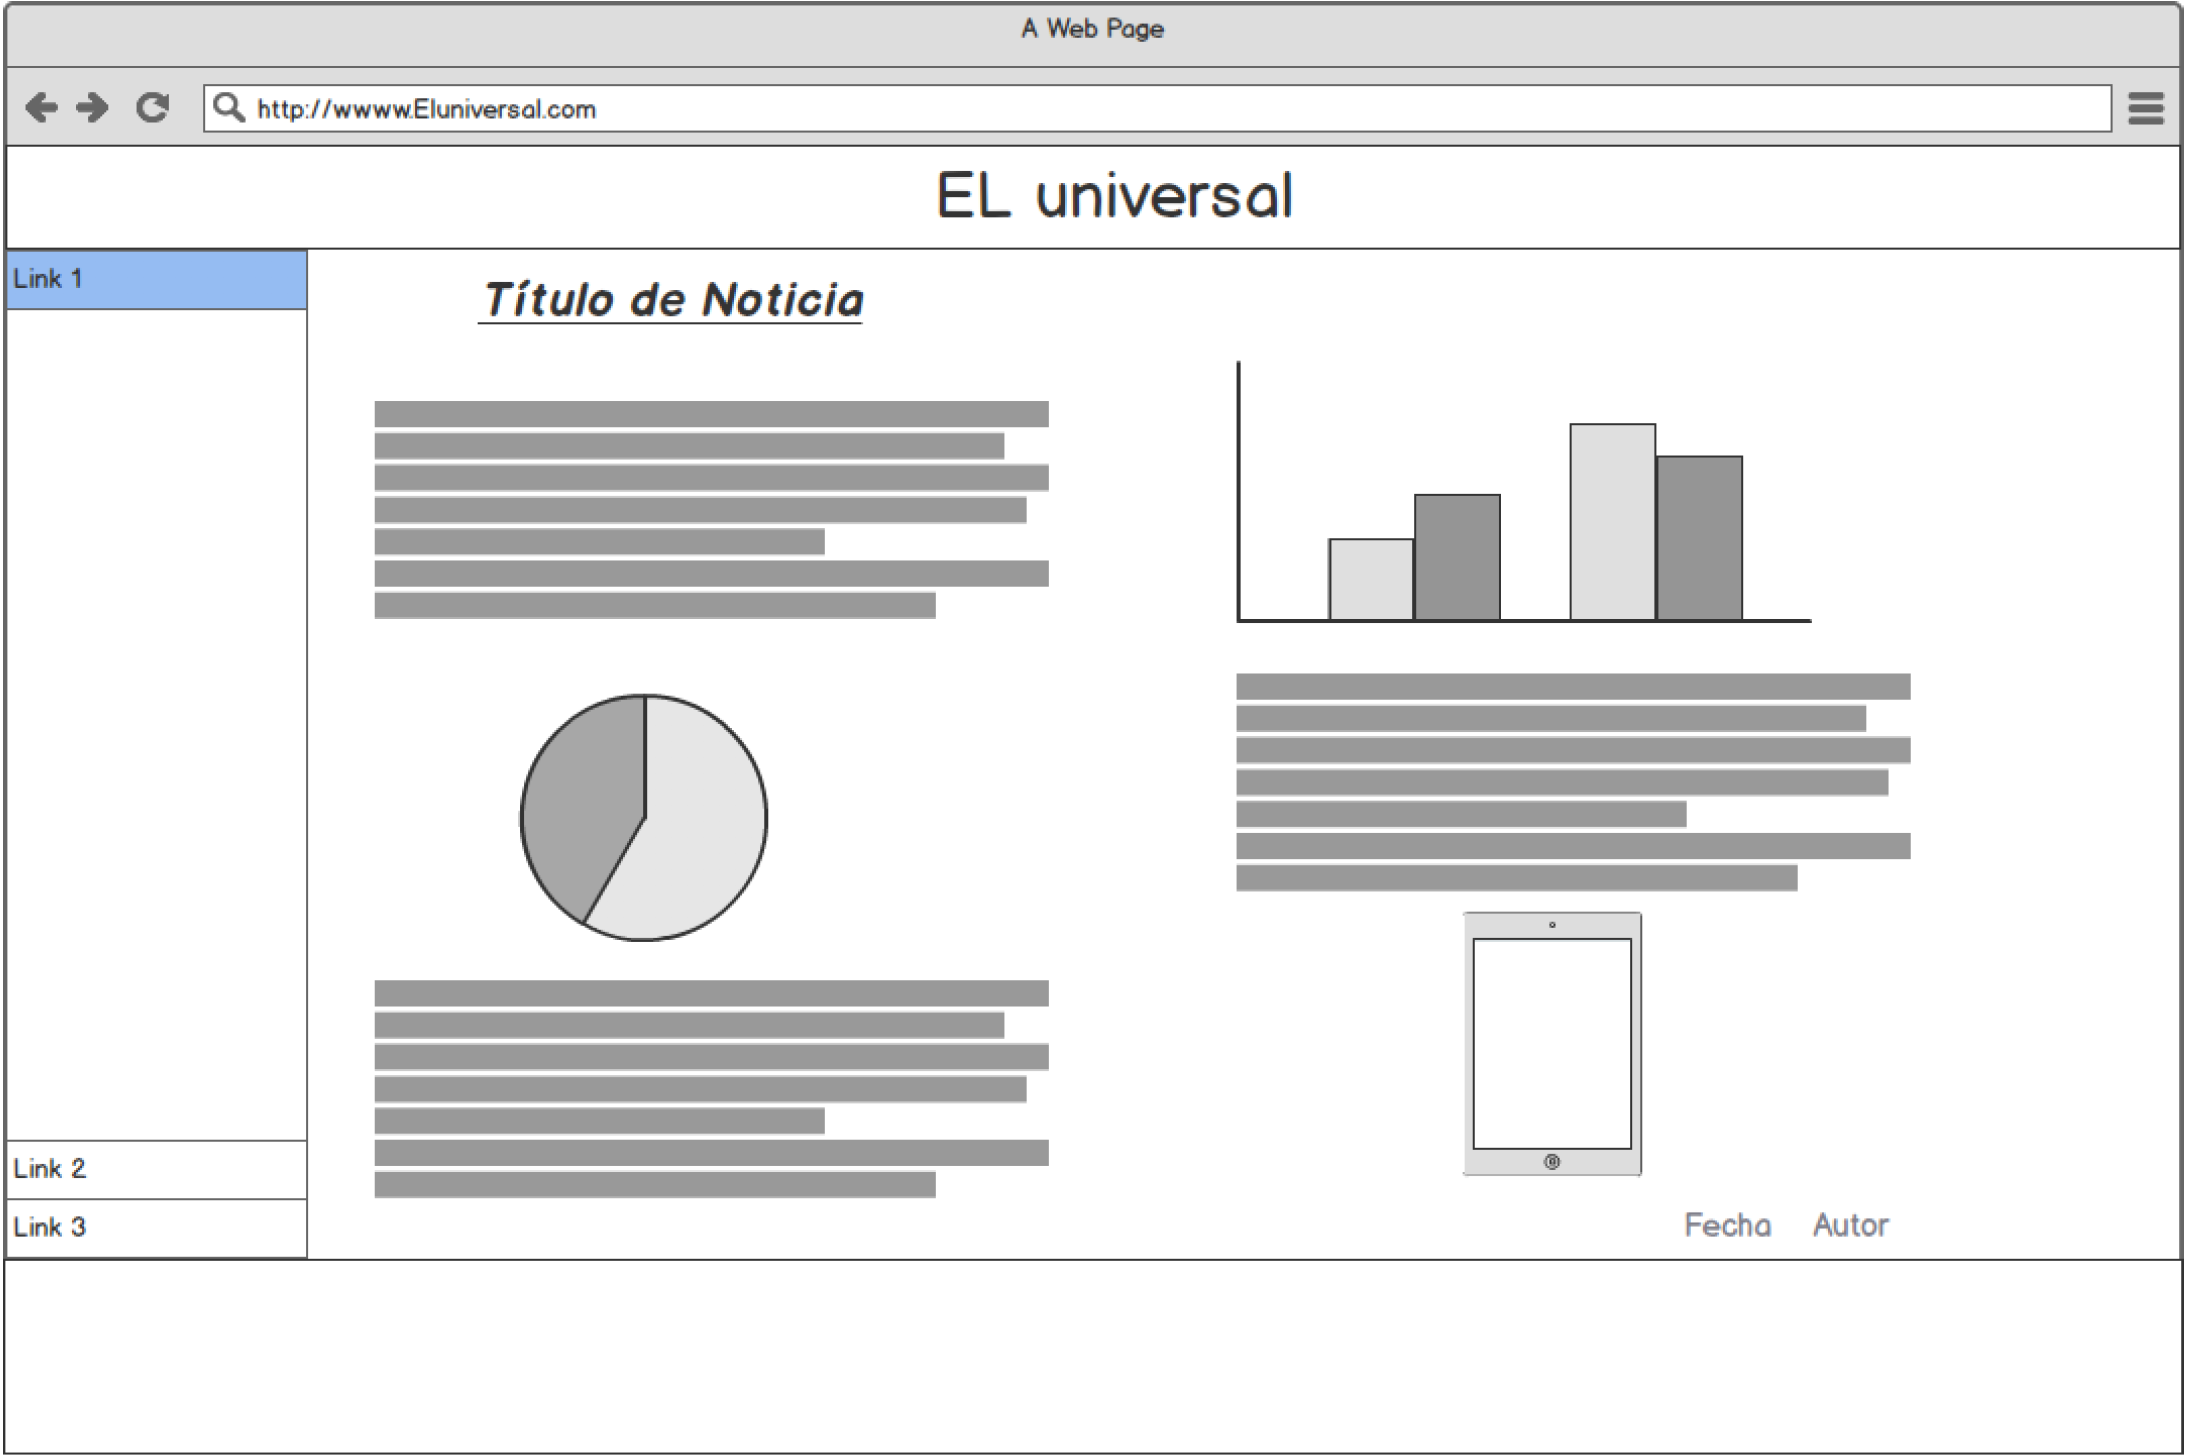
\includegraphics[scale=.3]{imagenes/Pantallas/UI4}
  \caption{Pantalla IU4-Página ejemplo}
  \label{fig:IU4}
\end{figure}
\newpage




